\section{Introdução}

  \subsection{Objetivo}
  O objetivo desse documento é especificar os casos de uso do projeto \ipPROCESSProject. O documento contempla as seguintes informações: descrição dos Atores envolvidos no processo; definição dos fluxos de eventos principal e secundário; lista de requisitos essenciais, funcionais e não funcionais; estabelecimento de pré-condições e pós-condições.

  \subsection{Visão Geral do Documento}
  \begin{itemize}
    \item Sessão 2: lista todos os possíveis atores do sistema.
    \item Sessão 3: relata a lista dos casos de uso do projeto.
    % \item Referências: provê uma lista completa de todos os artefatos referenciados nesse documento.
  \end{itemize}
  
  \subsection{Representação Simbólica}
  A Figura \ref{fig:uc_exemple} ilustra a simbologia utilizada para representar operações que devem ser realizadas pelo sistema. A Figura \ref{fig:actors} ilustra as duas simbologias utilizadas para representar os Atores do sistema. Um ator, dentro do escopo desta descrição, pode ser identificado como um módulo \textit{top level}, ou como um elemento de entrada e saída (botões, sensores, displays, etc).
  
  % \FloatBarrier
  % \begin{figure}[H]
  %   \centering
  %   
\includegraphics[width=0.25\textwidth]{uc_exemple.png}
  %   \caption{Exemplo de Caso de Uso.}
  %   \label{fig:uc_exemple}
  % \end{figure}
    \begin{figure}[H]
      \centering
      \begin{tikzpicture} 
        \umlusecase[name=usecase]{Caso de Uso}
      \end{tikzpicture}  
      \caption{Exemplo de Caso de Uso.}
      \label{fig:uc_exemple}
    \end{figure}
  
  A simbologia usual para representação de um Ator é apresentada na Figura \ref{fig:actor_exemple}, no entanto, para representar módulos incorporados que outrora deveriam utilizar a mesma simbologia, utiliza-se a representação ilustrada nas Figuras \ref{fig:ipcore_exemple} e \ref{fig:ipcore_single_exemple}, definida por convenção. Este elemento, em geral, está associado aos módulos do sistema, ou IP-cores que de terceiros incorporados ao mesmo. Esta simbologia ainda foi divida, tendo em vista representar instâncias únicas (Figura \ref{fig:ipcore_single_exemple}), ou múltiplas (Figura \ref{fig:ipcore_exemple}) de um determinado componente. 
  
  \FloatBarrier
  \begin{figure}[H]
    \centering
    \begin{subfigure}[b]{0.3\textwidth}
      \centering
      \begin{tikzpicture} 
        \umlactor{Ator}
      \end{tikzpicture}
      \caption{Ator do Sistema.}
      \label{fig:actor_exemple}
    \end{subfigure} 
    \begin{subfigure}[b]{0.3\textwidth}
      \centering
      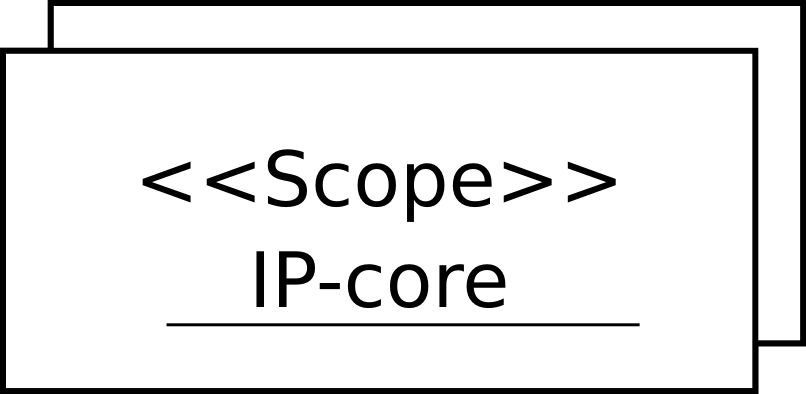
\includegraphics[width=0.6\textwidth]{ipcore_exemple.png}
      \caption{Instância múltipla de um IP.}
      \label{fig:ipcore_exemple}
    \end{subfigure}
    \begin{subfigure}[b]{0.3\textwidth}
      \centering
      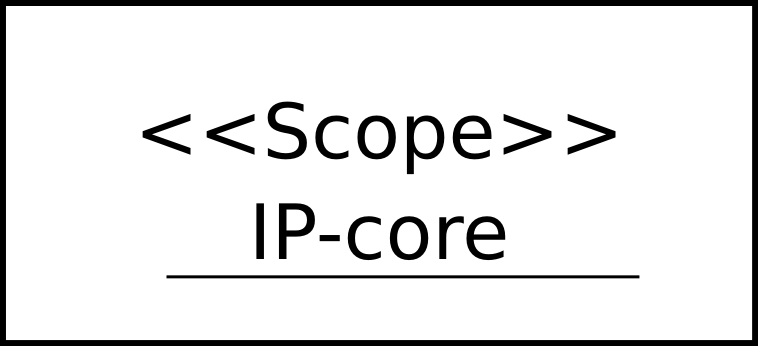
\includegraphics[width=0.6\textwidth]{ipcore_single_exemple.png}
      \caption{Instância de um IP.}
      \label{fig:ipcore_single_exemple}
    \end{subfigure}
    \caption{Simbologia utilizada na implementação dos Casos de Uso.}
    \label{fig:actors}
  \end{figure}
  
  O projetista responsável por interpretar os diagramas não deve confundir-se no momento de interpretar as simbologias de atores. A representação alternativa, não implica que o módulo será instanciado no subsistema em questão, mas sim que os recursos providos por este \textit{core} são necessários para garantir o seu funcionamento.
  
  \subsection{Definições, Acrônimos e Abreviações}
  \FloatBarrier
    \begin{table}[H] 
      \begin{center}
        \begin{tabular}[pos]{|m{2cm} | m{8cm}|} 
          \hline \cellcolor[gray]{0.9}\textbf{Termo} & \cellcolor[gray]{0.9}\textbf{Descrição} \\ \hline
          UC & Caso de Uso  \\ \hline
%         SF & Fluxo Secundário \\ \hline
          %FR & Requisito Funcional \\ \hline
          IF & Busca de Instrução \\ \hline
          ID & Decodificação de Instrução \\ \hline 
          EX & Execução \\ \hline 
          MEM/WB & Acesso a Memória/Escrita \\ \hline
          %DM & Memória de Dados \\ \hline
        \end{tabular}
      \end{center}
    \label{tab:definicoes}
    \end{table}